\chapter{Video Reconstruction}
\label{ch:video}
In this chapter, we explain how to use the MSCE algorithm in \cite{pilikos2014} to reconstruct masked video signals.

Throughout this chapter, we assume that $\bm v$ is a video signal of size $r\times c\times f$ ($r$ rows, $c$ columns and $f$ frames), where $r=2^{q_1}$, $c=2^{q_2}$ and $f=2^{q_3}$.

First, we explain how to extend the basis functions that were discussed in Chapter \ref{ch:dwt} to three dimensions.

\section{Three-Dimensional Basis Functions}
\subsection{Haar Wavelets for Videos}
A straightforward way of approaching the Discrete Wavelet Transform of a video would be to simply perform the two-dimensional DWT on each individual frame. 
This ``pseudo 3D'' approach is relatively simple, but typically also very inefficient.
Usually, we expect there to be continuity between successive frames of a video.
The pseudo 3D approach does not allow us to exploit any of the temporal correlations that are common in video signals.

A better approach would be to perform a full 3-D wavelet decomposition using three-dimensional scaling and wavelet functions.
In 3-D, we have one scaling function $\phi(x,y,t)$ and a total of $2^3-1=7$ wavelet functions.
These can be obtained by multiplying the 2-D functions in (\ref{eqn:2d_haar_wavelets}) with the scaling function $\phi(t)$ and the wavelet function $\psi(t)$ in the time domain:
\begin{equation*}
  \begin{split}
    \phi(x,y,t) &= \phi(t) \phi(x) \phi(y)\\
    \psi^H(x,y,t) &=\phi(t) \phi(x) \psi(y) \\
    \psi^V(x,y,t) &=\phi(t) \psi(x) \phi(y) \\
    \psi^D(x,y,t) &=\phi(t) \psi(x) \psi(y) \\
    \psi^T(x,y,t) &= \psi(t) \phi(x) \phi(y)\\
    \psi^{HT}(x,y,t) &=\psi(t) \phi(x) \psi(y) \\
    \psi^{VT}(x,y,t) &=\psi(t) \psi(x) \phi(y) \\
    \psi^{DT}(x,y,t) &=\psi(t) \psi(x) \psi(y)
  \end{split}
\end{equation*}
We use the $T$ superscript to denote the high-pass filters in the temporal direction.

\begin{figure}
\centering
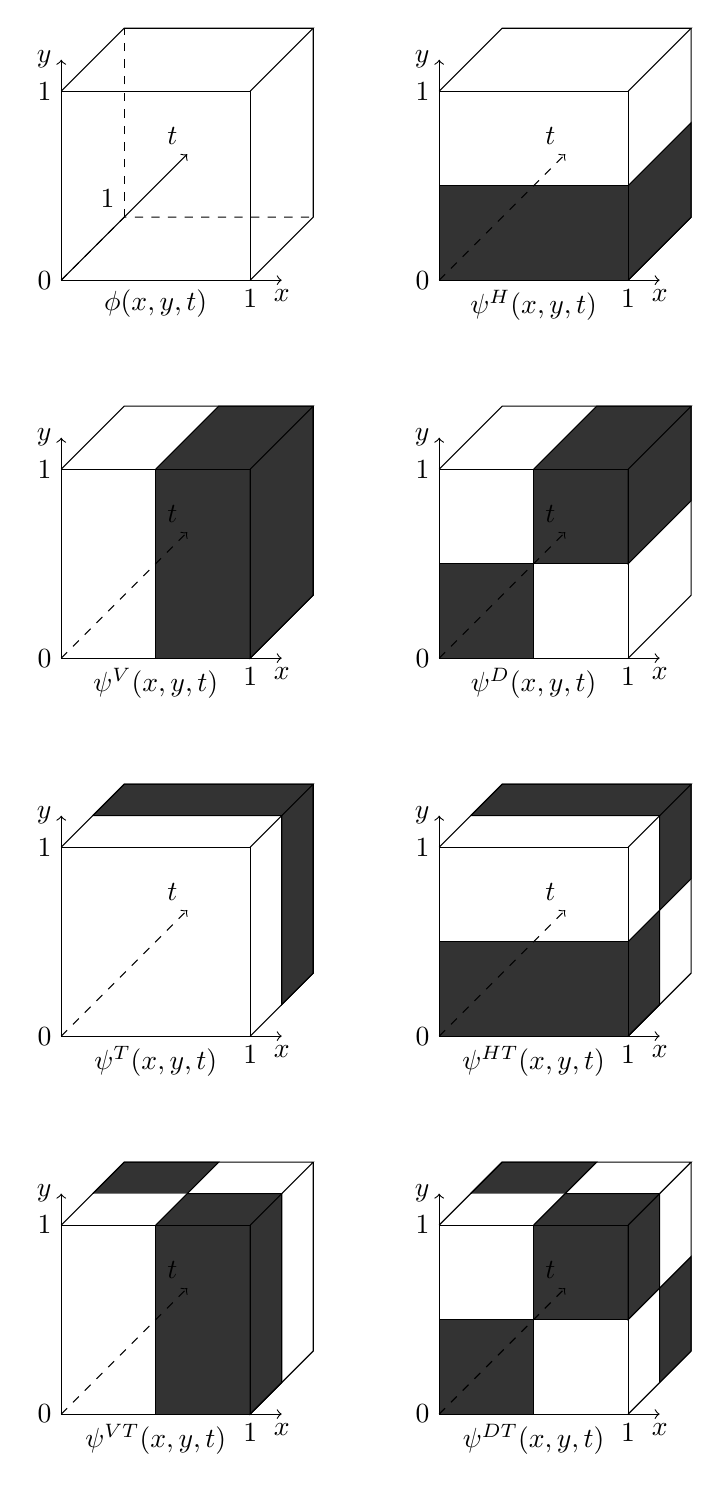
\begin{tikzpicture} [scale=0.8]
% top 4
  \draw [<->] (0,21.5) -- (0,18) -- (3.5,18);
  \draw [->] (0,18) -- (2,20);
  \draw (0,18) rectangle (3,21);
  \draw (0,21) -- (1,22) -- (4,22) -- (3,21);
  \draw (4,22) -- (4,19) -- (3,18);
  \draw [dashed] (0,18) -- (1,19) -- (4,19);
  \draw [dashed] (1,19) -- (1,22);

  \draw [<->] (6,21.5) -- (6,18) -- (9.5,18);
  \draw [->,dashed] (6,18) -- (8,20);
  \draw (6,18) rectangle (9,21);
  \draw (6,21) -- (7,22) -- (10,22) -- (9,21);
  \draw (10,22) -- (10,19) -- (9,18);

  \draw [<->] (0,15.5) -- (0,12) -- (3.5,12);
  \draw [->,dashed] (0,12) -- (2,14);
  \draw (0,12) rectangle (3,15);
  \draw (0,15) -- (1,16) -- (4,16) -- (3,15);
  \draw (4,16) -- (4,13) -- (3,12);

  \draw [<->] (6,15.5) -- (6,12) -- (9.5,12);
  \draw [->,dashed] (6,12) -- (8,14);
  \draw (6,12) rectangle (9,15);
  \draw (6,15) -- (7,16) -- (10,16) -- (9,15);
  \draw (10,16) -- (10,13) -- (9,12);
  
  \node at (1.5,18) [below] {$\phi(x,y,t)$};
  \node at (0,18) [left] {$0$};
  \node at (0,21) [left] {$1$};
  \node at (3,18) [below] {$1$};
  \node at (3.5,18) [below] {$x$};
  \node at (0,21.5) [left] {$y$};
  \node at (2,20) [above left] {$t$};
  \node at (1,19.3) [left] {$1$};
  
  \node at (7.5,18) [below] {$\psi^H(x,y,t)$};
  \node at (6,18) [left] {$0$};
  \node at (6,21) [left] {$1$};
  \node at (9,18) [below] {$1$};
  \node at (9.5,18) [below] {$x$};
  \node at (6,21.5) [left] {$y$};
  \node at (8,20) [above left] {$t$};

  \node at (1.5,12) [below] {$\psi^V(x,y,t)$};
  \node at (0,12) [left] {$0$};
  \node at (0,15) [left] {$1$};
  \node at (3,12) [below] {$1$};
  \node at (3.5,12) [below] {$x$};
  \node at (0,15.5) [left] {$y$};
  \node at (2,14) [above left] {$t$};

  \node at (7.5,12) [below] {$\psi^D(x,y,t)$};
  \node at (6,12) [left] {$0$};
  \node at (6,15) [left] {$1$};
  \node at (9,12) [below] {$1$};
  \node at (9.5,12) [below] {$x$};
  \node at (6,15.5) [left] {$y$};
  \node at (8,14) [above left] {$t$};

%bottom 4
  \draw [<->] (0,9.5) -- (0,6) -- (3.5,6);
  \draw [->,dashed] (0,6) -- (2,8);
  \draw (0,6) rectangle (3,9);
  \draw (0,9) -- (1,10) -- (4,10) -- (3,9);
  \draw (4,10) -- (4,7) -- (3,6);
  
  \draw [<->] (6,9.5) -- (6,6) -- (9.5,6);
  \draw [->,dashed] (6,6) -- (8,8);
  \draw (6,6) rectangle (9,9);
  \draw (6,9) -- (7,10) -- (10,10) -- (9,9);
  \draw (10,10) -- (10,7) -- (9,6);

  \draw [<->] (0,3.5) -- (0,0) -- (3.5,0);
  \draw [->,dashed] (0,0) -- (2,2);
  \draw (0,0) rectangle (3,3);
  \draw (0,3) -- (1,4) -- (4,4) -- (3,3);
  \draw (4,4) -- (4,1) -- (3,0);

  \draw [<->] (6,3.5) -- (6,0) -- (9.5,0);
  \draw [->,dashed] (6,0) -- (8,2);
  \draw (6,0) rectangle (9,3);
  \draw (6,3) -- (7,4) -- (10,4) -- (9,3);
  \draw (10,4) -- (10,1) -- (9,0);
  
  \node at (1.5,6) [below] {$\psi^T(x,y,t)$};
  \node at (0,6) [left] {$0$};
  \node at (0,9) [left] {$1$};
  \node at (3,6) [below] {$1$};
  \node at (3.5,6) [below] {$x$};
  \node at (0,9.5) [left] {$y$};
  \node at (2,8) [above left] {$t$};

  \node at (7.5,6) [below] {$\psi^{HT}(x,y,t)$};
  \node at (6,6) [left] {$0$};
  \node at (6,9) [left] {$1$};
  \node at (9,6) [below] {$1$};
  \node at (9.5,6) [below] {$x$};
  \node at (6,9.5) [left] {$y$};
  \node at (8,8) [above left] {$t$};

  \node at (1.5,0) [below] {$\psi^{VT}(x,y,t)$};
  \node at (0,0) [left] {$0$};
  \node at (0,3) [left] {$1$};
  \node at (3,0) [below] {$1$};
  \node at (3.5,0) [below] {$x$};
  \node at (0,3.5) [left] {$y$};
  \node at (2,2) [above left] {$t$};

  \node at (7.5,0) [below] {$\psi^{DT}(x,y,t)$};
  \node at (6,0) [left] {$0$};
  \node at (6,3) [left] {$1$};
  \node at (9,0) [below] {$1$};
  \node at (9.5,0) [below] {$x$};
  \node at (6,3.5) [left] {$y$};
  \node at (8,2) [above left] {$t$};
  % fills
  % top
  %TH
  \draw [fill=black, fill opacity=0.8] (6,18) rectangle (9,19.5);
  \draw [fill=black, fill opacity=0.8] (9,19.5) -- (10,20.5) -- (10,19) -- (9,18);
 
  % V
  \draw [fill=black, fill opacity=0.8] (1.5,12) rectangle (3,15);
  \draw [fill=black, fill opacity=0.8] (1.5,15) -- (2.5,16) -- (4,16) -- (4,13) -- (3,12) -- (3,15);

  %TD
  \draw [fill=black, fill opacity=0.8] (6,12) rectangle (7.5,13.5);
  \draw [fill=black, fill opacity=0.8] (7.5,13.5) rectangle (9,15);
  \draw [fill=black, fill opacity=0.8] (7.5,15) -- (8.5,16) -- (10,16) -- (10,14.5) -- (9,13.5) -- (9,15);
    
  % bottom
  % T
  \draw [fill=black, fill opacity=0.8] (0.5,9.5) -- (1,10) -- (4,10) -- (4,7) -- (3.5,6.5) -- (3.5,9.5) -- (0.5,9.5);
  %TH
  \draw [fill=black, fill opacity=0.8] (6,6) rectangle (9,7.5);
  \draw [fill=black, fill opacity=0.8] (6.5,9.5) -- (7,10) -- (10,10) -- (10,8.5) -- (9.5,8) -- (9.5,9.5) -- (6.5,9.5);
  \draw [fill=black, fill opacity=0.8] (9,7.5) -- (9.5,8) -- (9.5,6.5) -- (9,6);
  %TV
  \draw [fill=black, fill opacity=0.8] (1.5,0) rectangle (3,3);
  \draw [fill=black, fill opacity=0.8] (1.5,3) -- (2,3.5) -- (3.5,3.5) -- (3.5,0.5) -- (3,0) -- (3,3);
  \draw [fill=black, fill opacity=0.8] (0.5,3.5) -- (1,4) -- (2.5,4) -- (2,3.5);
  %TD
  \draw [fill=black, fill opacity=0.8] (6,0) rectangle (7.5,1.5);
  \draw [fill=black, fill opacity=0.8] (7.5,1.5) rectangle (9,3);
  \draw [fill=black, fill opacity=0.8] (7.5,3) -- (8,3.5) -- (9.5,3.5) -- (9.5,2) -- (9,1.5) -- (9,3);
  \draw [fill=black, fill opacity=0.8] (9.5,0.5) -- (9.5,2) -- (10,2.5) -- (10,1);
  \draw [fill=black, fill opacity=0.8] (6.5,3.5) -- (7,4) -- (8.5,4) -- (8,3.5);
\end{tikzpicture}
\caption[3-D Haar Wavelets]{The 3-D Haar scaling function and wavelet functions.
  Inside the $[0,1]\times [0,1] \times [0,1]$ cube, white corresponds to $+1$ and black corresponds to $-1$.
The functions are zero outside of the cube.}
\label{fig:haar_3d}
\end{figure}

\begin{figure}
  \centering
  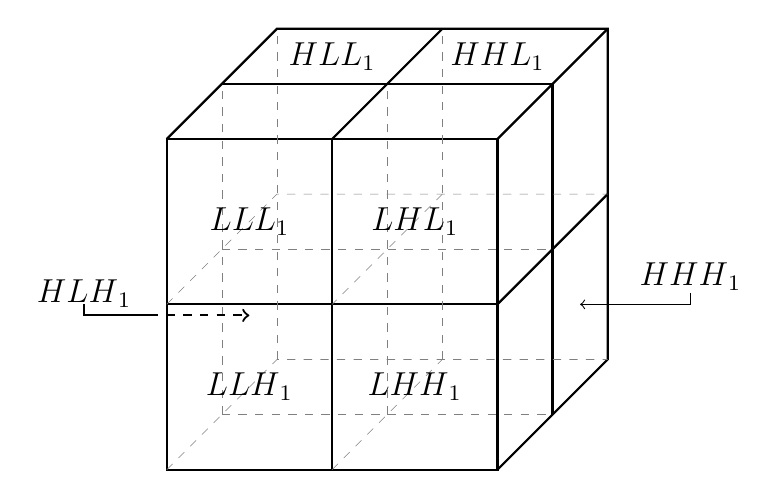
\begin{tikzpicture}[scale = 0.7]
    \draw [thick] (0,0) rectangle (6,6);
    \draw [thick] (0,3) -- (6,3);
    \draw [thick] (3,0) -- (3,6);
    \draw [thick] (0,6) -- (2,8) -- (8,8) -- (8,2) -- (6,0);
    \draw [thick] (1,7) -- (7,7) -- (7,1);
    \draw [thick] (6,6) -- (8,8);
    \draw [thick] (6,3) -- (8,5);
    \draw [thick] (3,6) -- (5,8);
    \draw [dashed,gray,very thin] (0,0) -- (2,2) -- (8,2);
    \draw [dashed,gray,very thin] (2,2) -- (2,8);
    \draw [dashed,gray,very thin] (1,1) -- (7,1);
    \draw [dashed,gray,very thin] (0,3) -- (2,5) -- (8,5);
    \draw [dashed,gray,very thin] (5,5) -- (3,3);
    \draw [dashed,gray,very thin] (1,4) -- (7,4);
    \draw [dashed,gray,very thin] (3,0) -- (5,2);
    \draw [dashed,gray,very thin] (4,1) -- (4,7);
    \draw [dashed,gray,very thin] (5,2) -- (5,8);
    \draw [dashed,gray,very thin] (1,1) -- (1,7);
    \node at (6,7.5) {\large$\bm{HHL}_1$};
    \node at (3,7.5) {\large$\bm{HLL}_1$};
    \node at (1.5,4.5) {\large$\bm{LLL}_1$};
    \node at (4.5,4.5) {\large$\bm{LHL}_1$};
    \node at (1.5,1.5) {\large$\bm{LLH}_1$};
    \node at (4.5,1.5) {\large$\bm{LHH}_1$};
    \node at (9.5,3.5) {\large$\bm{HHH}_1$};
    \draw [<-] (7.5,3) -- (9.5,3) -- (9.5,3.2);
    \node at (-1.5,3.2) {\large$\bm{HLH}_1$};
    \draw [thick](-1.5,3) -- (-1.5,2.8) -- (-0.3,2.8);
    \draw [->,dashed,thick] (-0.3,2.8) -- (1.5,2.8);
  \end{tikzpicture}
  \caption[Wavelet decomposition of a video]{The wavelet decomposition of a three-dimensional signal $v(x,y,t)$ at the first scale. 
    $L$ stands for ``low'' and $H$ stands for ``high''.
    To obtain the decomposition at higher scales, we recursively decompose the low-pass channels $\bm{LLL}_j$ in a similar way.}
  \label{fig:3d_channels}
\end{figure}

\begin{figure}
\centering
  \begin{subfigure}{0.35\textwidth}
    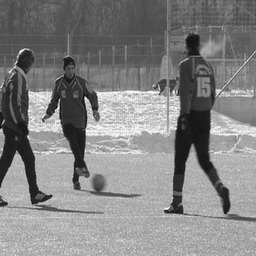
\includegraphics[width=0.9\textwidth]{Chapter3/Images/frame_11.png}
    \caption{Frame 11}
  \end{subfigure}
  \begin{subfigure}{0.35\textwidth}
    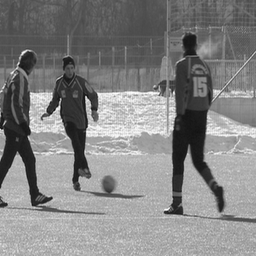
\includegraphics[width=0.9\textwidth]{Chapter3/Images/frame_12.png}
    \caption{Frame 12}
  \end{subfigure}
  \begin{subfigure}{0.35\textwidth}
    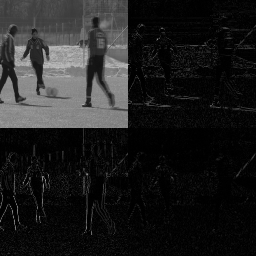
\includegraphics[width=0.9\textwidth]{Chapter3/Images/dwt_6.png}
    \caption{Scale 1 DWT: ``frame'' 6}
  \end{subfigure}
  \begin{subfigure}{0.35\textwidth}
    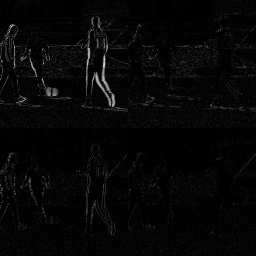
\includegraphics[width=0.9\textwidth]{Chapter3/Images/dwt_38.png}
    \caption{Scale 1 DWT: ``frame'' 38}
  \end{subfigure}
  \caption[Example showing the Haar wavelet decomposition of a video signal]{Frames 11 and 12 of a 64-frame video with a resolution of $256\times 256$ (a,b).
    We perform the three-dimensional DWT at the first scale using Haar wavelets and show two ``slices'' of the resulting coefficients (c,d). The detail coefficients have been enhanced to improve visibility.}
 \label{fig:3d_dwt}
\end{figure}

Figure \ref{fig:haar_3d} shows the 3-D scaling and wavelet functions for the Haar wavelets.
To obtain the basis functions corresponding to the 3-D Haar wavelet domain, we compute scaled and shifted versions of these functions as in:% (\ref{eqn:haar_scaling_basis}) and (\ref{eqn:haar_wavelet_basis}).
\begin{equation*}
  \phi_{k_1,k_2,k_3}^j(x,y,t) = 2^{3j/2} \phi(2^j t - k_3)\phi(2^j x - k_1) \phi(2^j y - k_2)
\end{equation*}

At the first scale, the 3-D wavelet decomposition of a video results in 8 channels: one corresponding to a low-pass filter, and 7 corresponding to high-pass filters in various directions (see Figure \ref{fig:3d_channels}).

For the Haar wavelets, the high-pass filters act as edge detectors, just like in the 2-D case. 
However, on top of detecting edges along spatial directions, we also get high-pass filters that detect sudden changes in the temporal direction, i.e. motion detectors.

As an example, consider Figure \ref{fig:3d_dwt}.
In panels (a) and (b), we show two adjacent frames of the ``soccer'' test video.
We perform the 3-D Haar DWT at the first scale and arrange the coefficients as in Figure \ref{fig:3d_channels}.
At the first scale, the 3-D Haar basis functions only have support over a $2\times 2\times 2$ volume.
Thus, all the DWT coefficients that are affected by the data in frames 11 and 12 of the original video, are contained within two ``frames'', or ``slices'', of the transformed signal.
For frames 11 and 12 of the original 64-frame video, these slices are at positions $12/2=6$ and $(6+64)/2=38$ in the transformed video.

In panel (c), we see the spatial edge detectors (the $LLH$, $LHL$ and $LHH$ channels) that are similar to those in the 2-D case (Figure \ref{fig:dwt2}).
The top left corner corresponds to the low-pass filter $LLL$ and can be regarded as an ``average'' of the video.

Panel (d), shows the four channels associated with a high-pass filter in the temporal direction.
The $HLL$ channel (top left corner of panel (d)) picks up overall differences in adjacent frames.
In this example, we note that it detects the motion of the football players and the ball, (as well as a slight motion of the backgrund due to the panning of the camera).
The remaining channels in panel (d) combine motion detection with edge detection.

\subsection{Three-Dimensional DCT}
The seperability property of the DCT makes the extension to three dimensions straightforward.
To compute the DCT of a video, we first compute the 2-D DCT for each individual frame of the video followed by a 1-D DCT across the temporal axis for each pixel.
The DCT basis functions (\ref{eqn:dct_basis}) in 3-D are characterised by a horizontal and vertical spatial frequency, as well as an additional temporal frequency component.

\section{Basis Matrix for Three-Dimensional Signals}
We vectorize $\bm v$ by first vectorizing each individual frame in a row-major fashion (see Section \ref{sect:vectorize2d}), followed by stacking the vectorized frames on top of each other.
The result $\bm v^V$ is a long vector of length $rcf$.

The basis matrix corresponding to the DCT is given by 
\begin{equation*}
  \bm\Psi = \bm\Psi_f\otimes\bm\Psi_c\otimes\bm\Psi_r
\end{equation*}
where $\bm\Psi_r$, $\bm\Psi_c$ and $\bm\Psi_f$ are the DCT basis matrices for 1-D signals (\ref{eqn:idct_basis}) of length $r$, $c$ and $f$, respectively.
See equation (\ref{eqn:kron}) for a definition of the Kronecker product $\otimes$.

The Haar basis matrix for video signals at scale 1 is constructed as follows:
\begin{equation*}
  \bm\Psi = 
  \begin{bmatrix}
    \bm H^{q_3}\otimes \bm H^{q_2} \otimes\bm H^{q_1} \\
    \bm H^{q_3}\otimes \bm H^{q_2} \otimes \bm G^{q_1} \\
    \bm H^{q_3}\otimes \bm G^{q_2} \otimes \bm H^{q_1} \\
    \bm H^{q_3}\otimes \bm G^{q_2} \otimes \bm G^{q_1} \\
    \bm G^{q_3}\otimes \bm H^{q_2} \otimes\bm H^{q_1} \\
    \bm G^{q_3}\otimes \bm H^{q_2} \otimes \bm G^{q_1} \\
    \bm G^{q_3}\otimes \bm G^{q_2} \otimes \bm H^{q_1} \\
    \bm G^{q_3}\otimes \bm G^{q_2} \otimes \bm G^{q_1} 
  \end{bmatrix}^T.
\end{equation*}
where the matrices $\bm H$ and $\bm G$ are defined in equations (\ref{eqn:haar_H}) and (\ref{eqn:haar_G}).

The extension to higher scales is similar to equation (\ref{eqn:haar2_fullbasis}).
We can build the matrix up until the $q$th scale, where $q=\min\{q_1,q_2,q_3\}$.
The full basis matrix is
\begin{equation*}
  \resizebox{.9\hsize}{!}{$
  \bm\Psi = 
  \begin{bmatrix}
    (\bm H^{q_3-q}\bm H^{q_3-q+1}\cdots\bm H^{q_3})\otimes (\bm H^{q_2-q}\bm H^{q_2-q+1}\cdots\bm H^{q_2}) \otimes (\bm H^{q_1-q}\bm H^{q_1-q+1}\cdots\bm H^{q_1}) \\
    (\bm H^{q_3-q}\bm H^{q_3-q+1}\cdots\bm H^{q_3})\otimes (\bm H^{q_2-q}\bm H^{q_2-q+1}\cdots\bm H^{q_2}) \otimes (\bm G^{q_1-q}\bm H^{q_1-q+1}\cdots\bm H^{q_1}) \\
    (\bm H^{q_3-q}\bm H^{q_3-q+1}\cdots\bm H^{q_3})\otimes (\bm G^{q_2-q}\bm H^{q_2-q+1}\cdots\bm H^{q_2}) \otimes (\bm H^{q_1-q}\bm H^{q_1-q+1}\cdots\bm H^{q_1}) \\
    (\bm H^{q_3-q}\bm H^{q_3-q+1}\cdots\bm H^{q_3})\otimes (\bm G^{q_2-q}\bm H^{q_2-q+1}\cdots\bm H^{q_2}) \otimes (\bm G^{q_1-q}\bm H^{q_1-q+1}\cdots\bm H^{q_1}) \\
    (\bm G^{q_3-q}\bm H^{q_3-q+1}\cdots\bm H^{q_3})\otimes (\bm H^{q_2-q}\bm H^{q_2-q+1}\cdots\bm H^{q_2}) \otimes (\bm H^{q_1-q}\bm H^{q_1-q+1}\cdots\bm H^{q_1}) \\
    (\bm G^{q_3-q}\bm H^{q_3-q+1}\cdots\bm H^{q_3})\otimes (\bm H^{q_2-q}\bm H^{q_2-q+1}\cdots\bm H^{q_2}) \otimes (\bm G^{q_1-q}\bm H^{q_1-q+1}\cdots\bm H^{q_1}) \\
    (\bm G^{q_3-q}\bm H^{q_3-q+1}\cdots\bm H^{q_3})\otimes (\bm G^{q_2-q}\bm H^{q_2-q+1}\cdots\bm H^{q_2}) \otimes (\bm H^{q_1-q}\bm H^{q_1-q+1}\cdots\bm H^{q_1}) \\
    (\bm G^{q_3-q}\bm H^{q_3-q+1}\cdots\bm H^{q_3})\otimes (\bm G^{q_2-q}\bm H^{q_2-q+1}\cdots\bm H^{q_2}) \otimes (\bm G^{q_1-q}\bm H^{q_1-q+1}\cdots\bm H^{q_1}) \\
    (\bm H^{q_3-q+1}\bm H^{q_3-q+2}\cdots\bm H^{q_3})\otimes (\bm H^{q_2-q+1}\bm H^{q_2-q+2}\cdots\bm H^{q_2}) \otimes (\bm G^{q_1-q+1}\bm H^{q_1-q+2}\cdots\bm H^{q_1}) \\
    (\bm H^{q_3-q+1}\bm H^{q_3-q+2}\cdots\bm H^{q_3})\otimes (\bm G^{q_2-q+1}\bm H^{q_2-q+2}\cdots\bm H^{q_2}) \otimes (\bm H^{q_1-q+1}\bm H^{q_1-q+2}\cdots\bm H^{q_1}) \\
    \vdots\\
    (\bm G^{q_3-1}\bm H^{q_3})\otimes (\bm G^{q_2-1}\bm H^{q_2}) \otimes (\bm G^{q_1-1}\bm H^{q_1}) \\
    \bm H^{q_3}\otimes \bm H^{q_2} \otimes \bm G^{q_1} \\
    \bm H^{q_3}\otimes \bm G^{q_2} \otimes \bm H^{q_1} \\
    \bm H^{q_3}\otimes \bm G^{q_2} \otimes \bm G^{q_1} \\
    \bm G^{q_3}\otimes \bm H^{q_2} \otimes \bm H^{q_1} \\
    \bm G^{q_3}\otimes \bm H^{q_2} \otimes \bm G^{q_1} \\
    \bm G^{q_3}\otimes \bm G^{q_2} \otimes \bm H^{q_1} \\
    \bm G^{q_3}\otimes \bm G^{q_2} \otimes \bm G^{q_1} 
  \end{bmatrix}^T
$}
\end{equation*}

The size of the basis matrices is $(rcf)\times (rcf)$. 
Even for relatively small signals, these matrices can be prohibitively large.
We address this problem in Chapter \ref{ch:code}.


\section{Video Interpolation}
Once we have successfully created a vectorization scheme for the video signal $\bm v$ and constructed the Haar basis matrices $\bm\Psi$ for the desired scales, we can apply to MSCE to reconstruct masked video signals.

\begin{figure}
  \centering
  \textbf{\hspace{0.5in} Frame 21 \hspace{1.5in} Frame 151\hspace{0.5in}\vspace{0.2in}}
  \begin{subfigure}{0.4\textwidth}
    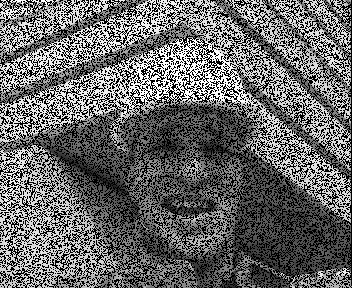
\includegraphics[width=\textwidth]{Chapter5/Images/foreman_masked_21.png}
    \caption{Corrupted}
  \end{subfigure}
  \begin{subfigure}{0.4\textwidth}
    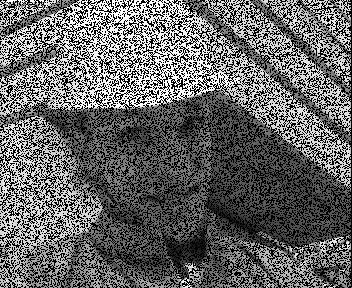
\includegraphics[width=\textwidth]{Chapter5/Images/foreman_masked_151.png}
    \caption{Corrupted}
  \end{subfigure}
  \begin{subfigure}{0.4\textwidth}
    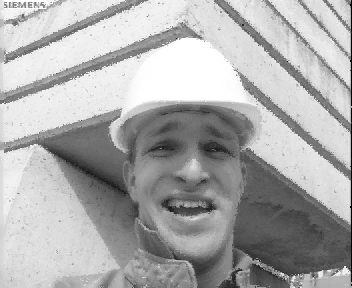
\includegraphics[width=\textwidth]{Chapter5/Images/foreman_rec_21.png}
    \caption{Recovered}
  \end{subfigure}
  \begin{subfigure}{0.4\textwidth}
    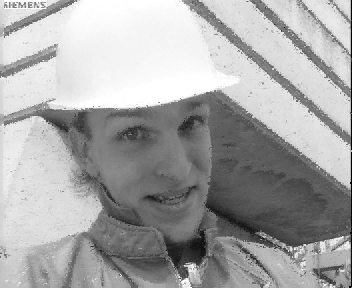
\includegraphics[width=\textwidth]{Chapter5/Images/foreman_rec_151.png}
    \caption{Recovered}
  \end{subfigure}
  \begin{subfigure}{0.4\textwidth}
    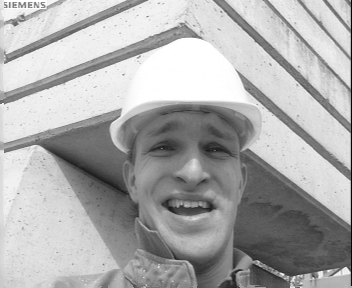
\includegraphics[width=\textwidth]{Chapter5/Images/foreman_orig_21.png}
    \caption{Original}
  \end{subfigure}
  \begin{subfigure}{0.4\textwidth}
    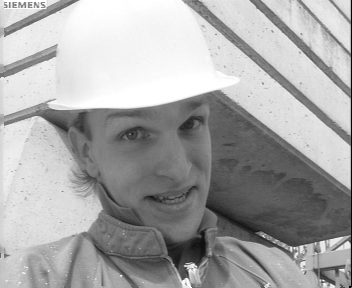
\includegraphics[width=\textwidth]{Chapter5/Images/foreman_orig_151.png}
    \caption{Original}
  \end{subfigure}
  \caption[Example output of our video interpolator]{Example of a masked video signal, where only 60\% of the pixel values are known (a-b). 
    Reconstruction via the MSCE Algorithm using 2 cascades (PSNR: 28.6) (c-d).
    Original video (e-f).}
  \label{fig:foreman_masked}
\end{figure}

We pass the measured pixel values $\bm y$ and the design matrix $\bm\Phi = \bm\Theta\bm\Psi$ (where $\bm\Theta$ is the video mask) t
o Algorithm \ref{alg3}.
The output will be an interpolated video that hopefully recovers very fine details across the entire signal.

Figure \ref{fig:foreman_masked}, we show two example frames of the test video ``foreman''.
Panels (a) and (b) show the undersampled signal $\bm y$.
Panels (c) and (d) show the output of the MSCE algorithm.
For reference, we have also included the frames from the original video in panels (e) and (f).

Further test results of this method are shown in Chapter \ref{ch:results}.

\section{Video Reconstruction from general CS measurements}
Unfortunetaly the MSCE don't work for general sensing matrices because it was designed specifically to deal with the problem of `black pixels vs blurriness'.

The problem is that the basis functions that the RVM works are actually (random) linear combinations of the DWT basis functions.
We want to get error bars on the reconstructed pixels, but the pixels are in a different ``domain'' as the CS measurements. 
So we cannot trust those errors.

If we can make additional measurements (random projection), we \emph{can} use the error bars to select optimal random projections \cite{ji2008}. 

To allow reconstruction of video from general CS measurements, we have also implemented the BCS algorithm [add alg box?].
In ch 8, we compare performance between different sensors (for masks, use both algorithms).
Also look at how block size and basis function choice affect performance for random sensors.